\chapter{Trigonometry}

\section{Sine, Cosine, and Tangent}
\begin{figure}[H]
  \begin{center}
    
\includegraphics[width=0.4\textwidth]{continuous/trig/basictrig}
  \end{center}
\end{figure}

For this example:
  \[\displaystyle{\sin\theta=\frac{b}{c}}\qquad
  \displaystyle{\cos\theta=\frac{a}{c}}\qquad
  \displaystyle{\tan\theta=\frac{b}{a}}\]
Gennerally speaking, for an angle $\theta$ on the inside of a right triangle,
\begin{itemize}
  \item$\sin\theta$ is equal to the \emph{length of the opposite side divided by the length of the hypotenuse\footnote{The hypotenuse is the side of a right triangle opposite the right angle.}}.
  \item$\cos\theta$ is equal to the \emph{adjacent side divided by the hypotenuse}.
  \item$\tan\theta$ is equal to the \emph{opposite over the adjacent side}.
\end{itemize}

\begin{figure}[h]
  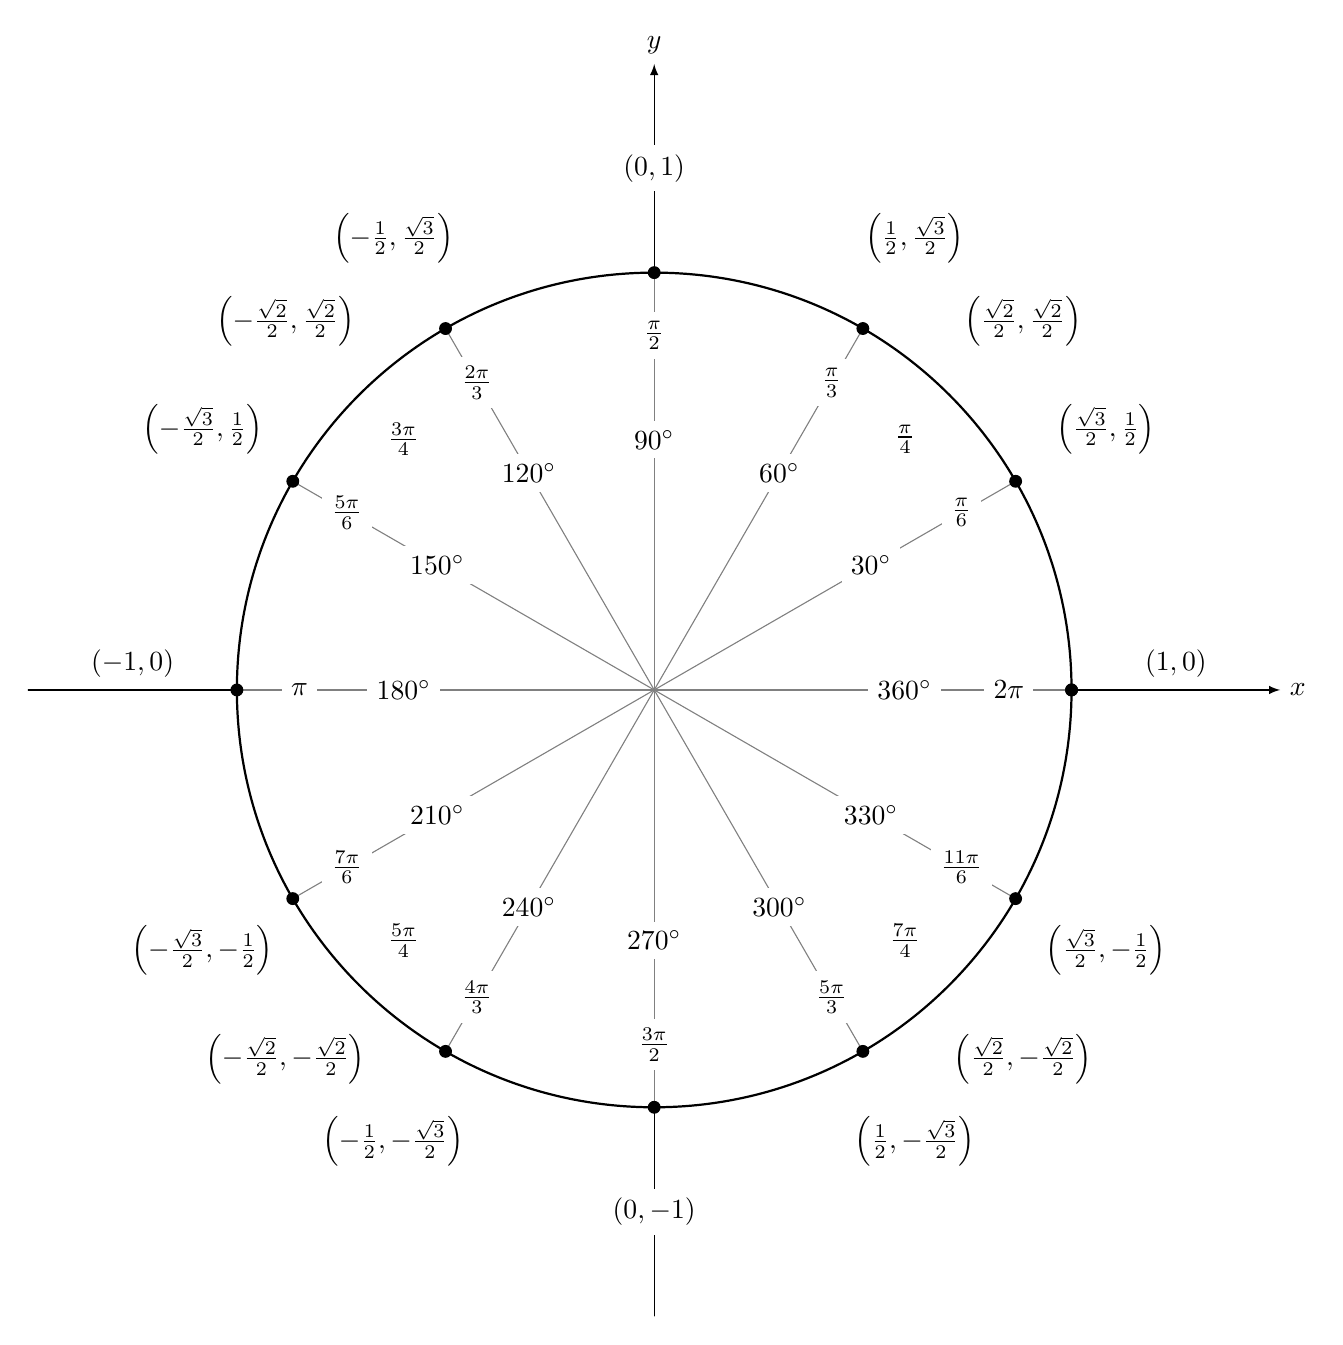
\begin{tikzpicture}[scale=5.3,cap=round,>=latex]
  % draw the coordinates
    \draw[->] (-1.5cm,0cm) -- (1.5cm,0cm) node[right,fill=white] {$x$};
    \draw[->] (0cm,-1.5cm) -- (0cm,1.5cm) node[above,fill=white] {$y$};

  % draw the unit circle
    \draw[thick] (0cm,0cm) circle(1cm);

    \foreach \x in {0,30,...,360} {
          % lines from center to point
      \draw[gray] (0cm,0cm) -- (\x:1cm);
          % dots at each point
      \filldraw[black] (\x:1cm) circle(0.4pt);
          % draw each angle in degrees
      \draw (\x:0.6cm) node[fill=white] {$\x^\circ$};
    }

  % draw each angle in radians
    \foreach \x/\xtext in {
      30/\frac{\pi}{6},
      45/\frac{\pi}{4},
      60/\frac{\pi}{3},
      90/\frac{\pi}{2},
      120/\frac{2\pi}{3},
      135/\frac{3\pi}{4},
      150/\frac{5\pi}{6},
      180/\pi,
      210/\frac{7\pi}{6},
      225/\frac{5\pi}{4},
      240/\frac{4\pi}{3},
      270/\frac{3\pi}{2},
      300/\frac{5\pi}{3},
      315/\frac{7\pi}{4},
      330/\frac{11\pi}{6},
    360/2\pi}
    \draw (\x:0.85cm) node[fill=white] {$\xtext$};

    \foreach \x/\xtext/\y in {
      % the coordinates for the first quadrant
      30/\frac{\sqrt{3}}{2}/\frac{1}{2},
      45/\frac{\sqrt{2}}{2}/\frac{\sqrt{2}}{2},
      60/\frac{1}{2}/\frac{\sqrt{3}}{2},
      % the coordinates for the second quadrant
      150/-\frac{\sqrt{3}}{2}/\frac{1}{2},
      135/-\frac{\sqrt{2}}{2}/\frac{\sqrt{2}}{2},
      120/-\frac{1}{2}/\frac{\sqrt{3}}{2},
      % the coordinate on s for the third quadrant
      210/-\frac{\sqrt{3}}{2}/-\frac{1}{2},
      225/-\frac{\sqrt{2}}{2}/-\frac{\sqrt{2}}{2},
      240/-\frac{1}{2}/-\frac{\sqrt{3}}{2},
      % the coordinates for the fourth quadrant
      330/\frac{\sqrt{3}}{2}/-\frac{1}{2},
      315/\frac{\sqrt{2}}{2}/-\frac{\sqrt{2}}{2},
      300/\frac{1}{2}/-\frac{\sqrt{3}}{2}}
      \draw (\x:1.25cm) node[fill=white] {$\left(\xtext,\y\right)$};

  % draw the horizontal and vertical coordinates
  % the placement is better this way
      \draw (-1.25cm,0cm) node[above=1pt] {$(-1,0)$}
      (1.25cm,0cm)  node[above=1pt] {$(1,0)$}
      (0cm,-1.25cm) node[fill=white] {$(0,-1)$}
      (0cm,1.25cm)  node[fill=white] {$(0,1)$};
  \end{tikzpicture}
  \caption{The unit circle, thanks to \cite{tikzunitcirc}.\label{fig:tikzunitcirc}}
\end{figure}


\section{Trigonometric Identities}\index{trigonometric identities}
Our first pythagorean identity is just derived from the pythagorean theorem.
\begin{theorem}
  In any right triangle, the area of the square whose side is the hypotenuse (the side opposite the right angle) is equal to the sum of the areas of the squares whose sides are the two legs (the two sides that meet at a right angle).
  %credit: wikipedia. Anyone have a better source?
  \label{th:pythagoras}
\end{theorem}
\begin{figure}[h]
  \begin{center}
    \subfigure[The Pythagorean Theorem states that the sum of the areas square $a$ and square $b$ is equal to the area of square $c$.]{\
      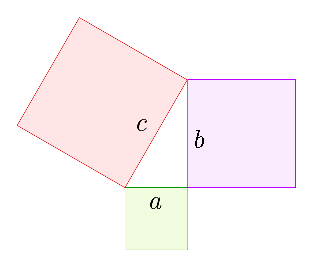
\includegraphics[width=0.4\textwidth]{continuous/functions/pyth}
      \label{fig:pyth}
    }
    \hspace{0.1\textwidth}
    \subfigure[The equation for a unit circle is $a^2+b^2=1$. This creates a circle with a radius of $1$.]{\
      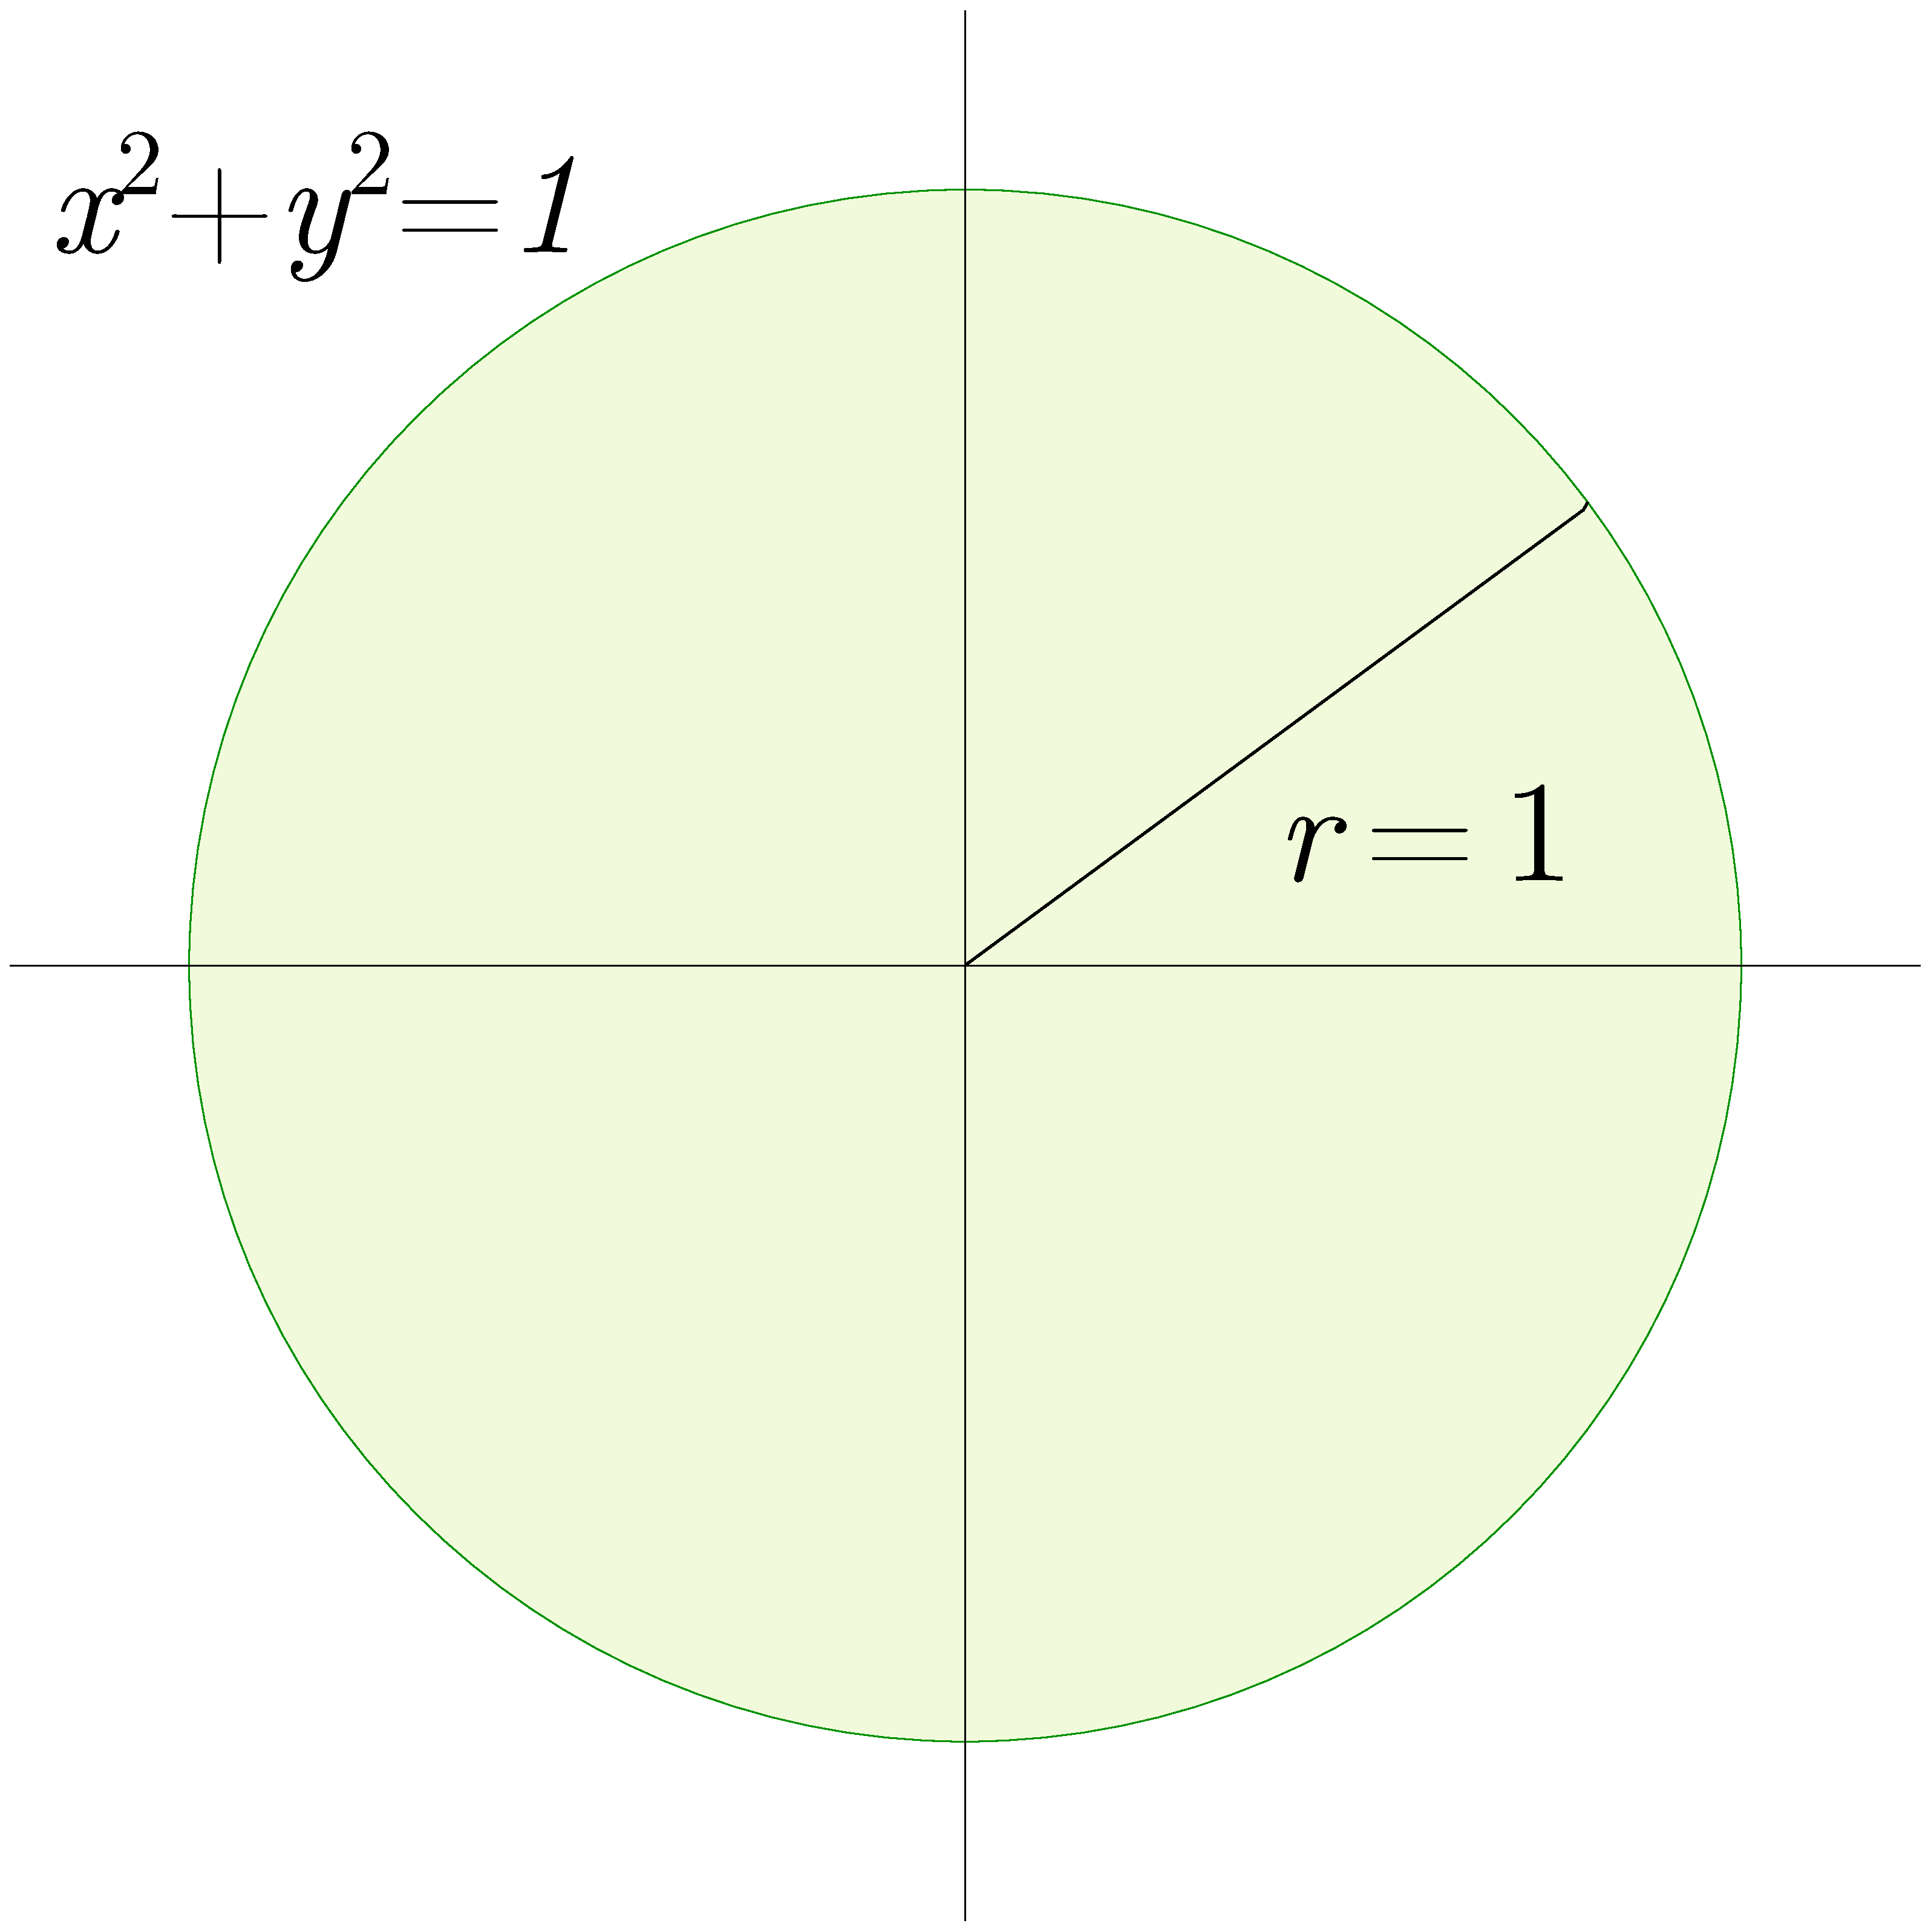
\includegraphics[width=0.4\textwidth]{continuous/functions/unitcirc}
      \label{fig:basicuniticircle}
    }
  \end{center}
\end{figure}
\begin{figure}[h]
  \begin{center}
    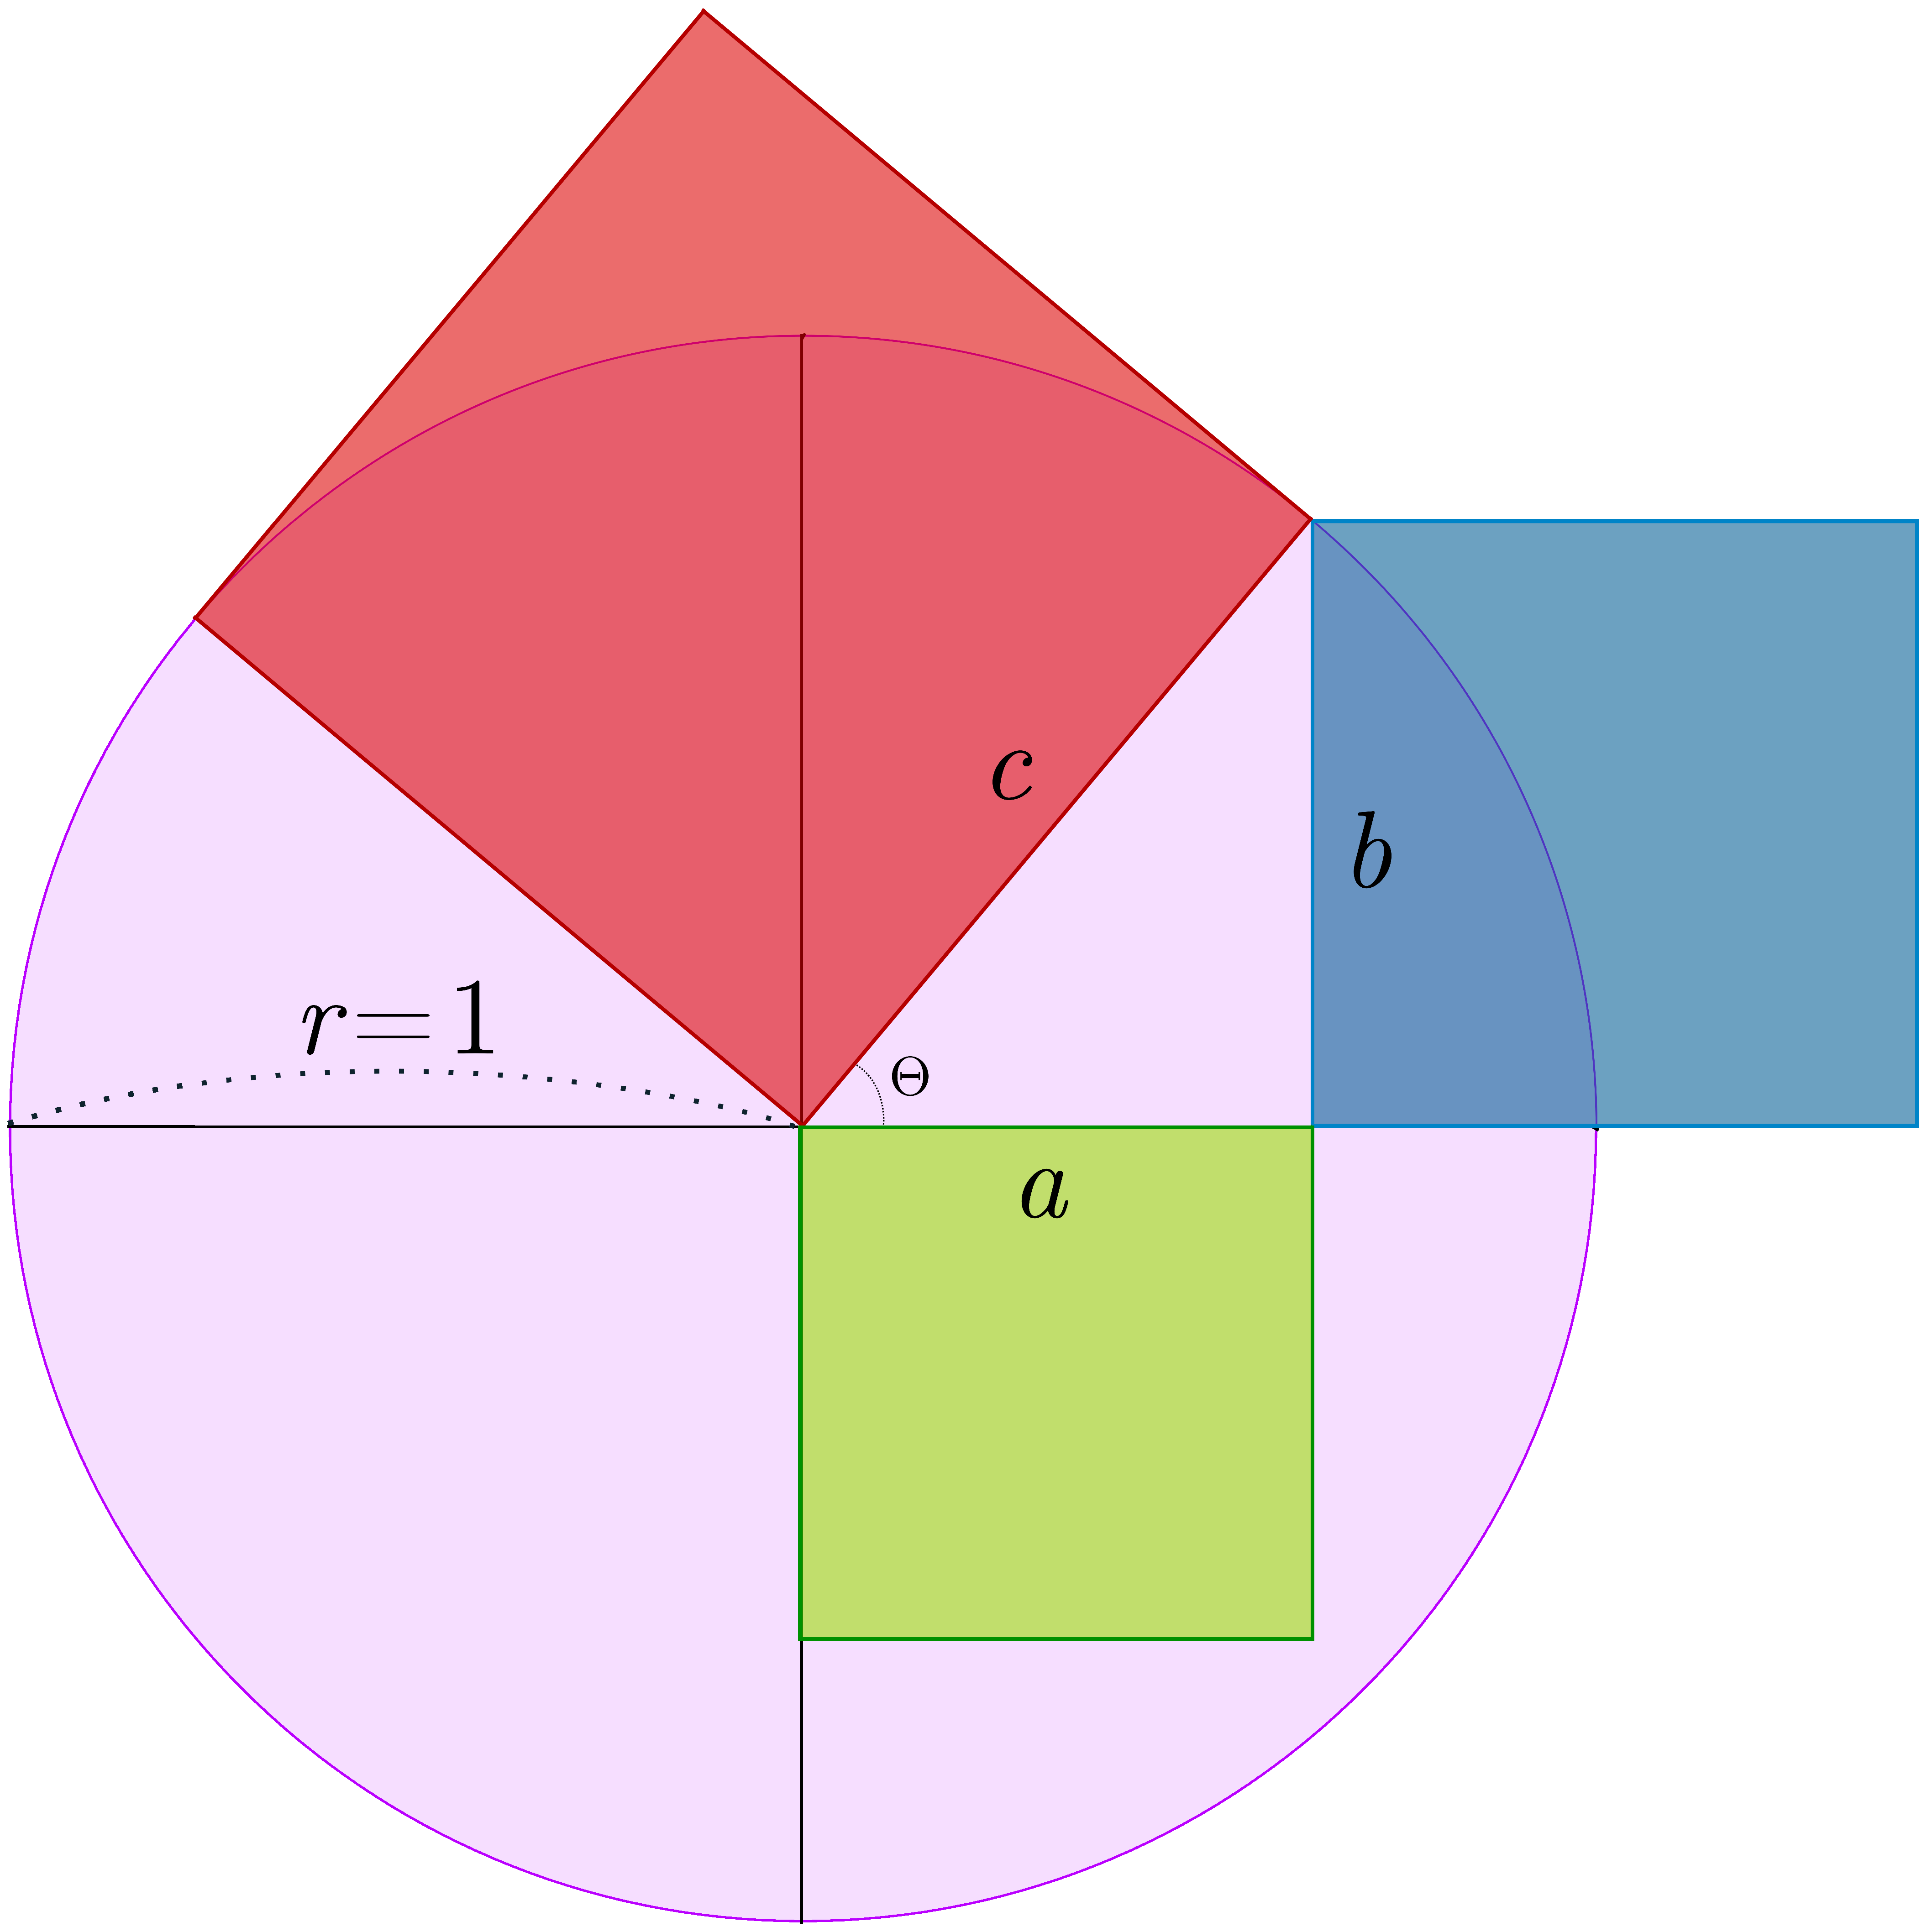
\includegraphics[width=0.5\textwidth]{continuous/trig/pythcircle}
    \caption{The pythagorean squares on a unit circle. Note that the length of side $c$ must be $1$ because the radius of the circle is $1$.}
  \end{center}
  \label{fig:pythcircle}
\end{figure}
Because the radius of the circle is $1$, then the length of side $c$ must also equal $1$.
From this, we can conclude that $\sin^2x+\cos^2x$ must, indeed, equal 1.

Why? From the picture, it is clear that both $c$ and $r$ are equal to $1$. Using the pythagorean theorem (theorem~\ref{th:pythagoras}):
\begin{proof}\begin{align*}
  a^2+b^2&=c^2\\
  a\cdot a + b \cdot b &= c \cdot c \\
  \intertext{we divide both sides by 1}
  \frac{b}{1}\cdot\frac{b}{1}+\frac{a}{1}\cdot\frac{a}{1}
  &=\frac{c \cdot c}{1}\\
  \intertext{because $c=1$}
  \frac{b}{c}\cdot\frac{b}{c}+\frac{a}{c}\cdot\frac{a}{c}
  &=1\\
  \intertext{remembering our definitions of sine and cosine}
  \sin\theta \cdot \sin\theta + \cos\theta \cdot \cos\theta &=1\\
  \sin^2\theta + \cos^2\theta &=1\qedhere
\end{align*}\end{proof}
We now have our first trigonometric identity.
\begin{equation}
  \sin^2x+\cos^2x=1
  \label{eq:pythtrig}
\end{equation}
The other ones, we either have to memorize or learn to derive (described in Section \ref{sec:trigderiv}).
\begin{equation}
  \sin{(x+y)} = \sin x \cos y + \sin y \cos x
\end{equation}
\begin{equation}
  \sin{(x-y)} = \sin x \cos y - \sin y \cos x
\end{equation}
\begin{equation}
  \cos(x+y)=\cos x \cos y - \sin x \sin y
  \label{eq:cosxpy}
\end{equation}
\begin{equation}
  \cos(x-y)=\cos x \cos y + \sin x \sin y
\end{equation}
\begin{equation}
  \sin{-x}=-\sin x
\end{equation}
\begin{equation}
  \sin{-x}=-\sin x
\end{equation}
\begin{equation}
  \sin{2x}=2 \big( \sin x \cos x \big)
\end{equation}
\begin{equation}
  \cos{2x}=\cos^2x-\sin^2x
\end{equation}

\section{Useful Trigonometric Relationships}\index{trigonometric relationships}
\begin{align}
    \frac{1}{\sin\theta}&=\csc\theta \\
    \frac{\cos\theta}{\sin\theta}&=\cot\theta \\
    \frac{\sin\theta}{\cos\theta}&=\tan\theta \\
    \frac{1}{\cos\theta}&=\sec\theta
  \end{align}

\section{Deriving Trigonometric Identities}\index{deriving trigonometric identities}\label{sec:trigderiv}

We recall that using the pythagorean theorem and a triangle with a hypotenuse of length $1$, we can obtain our first trigonometric identity:
\begin{equation}
	\sin^2x+\cos^2x=1
  \label{eq:pyth}
\end{equation}
Dividing by $\sin^2x$ gives us:
\begin{align}
\frac{\sin^2x}{\sin^2x}+\frac{\cos^2x}{\sin^2x}&=\frac{1}{\sin^2x} \nonumber \\
	1+\cot^2x&=\csc^2x
\end{align}
Dividing by $\cos^2x$ produces:
\begin{align}
  \frac{\sin^2x}{\cos^2x}+\frac{\cos^2x}{\cos^2x}+=&\frac{1}{\cos^2x} \nonumber \\
	\tan^2x+1=&\sec^2x
\end{align}

We should memorize the following two identities:
\begin{equation}
  \sin{a+b}=\sin a \cos a + \sin b \cos b
  \label{eq:sinab}
\end{equation}
\begin{equation}
  \cos{a+b}=\cos a \cos b + \sin a \sin b
  \label{eq:cosab}
\end{equation}
From equation \eqref{eq:sinab} we can infer that, if both $a$ and $b$ are the same,
\begin{equation}
  \sin{2\theta}=2 \sin \theta \cos \theta
  \label{eq:sin2q}
\end{equation}
using the same reasoning, \eqref{eq:cosab} gives us
\begin{align}
  \cos{2\theta}&=\cos \theta \cos \theta- \sin\theta \sin\theta \nonumber\\
  \cos{2\theta}&=\cos^2 \theta - \sin^2\theta
  \label{eq:cos2q}
\end{align}

We can generalize the pythagorean theorem by deriving the \textbf{law of cosines}\index{law of cosines}:
\begin{figure}[H]
  \begin{center}
    \includegraphics[width=0.4\textwidth]{continuous/trig/lawcosines}
  \end{center}
\end{figure}
In the above figure, we use the distance formula
\begin{equation}
  d=\sqrt{(x_1 - x_2)^2+(y_1-y_2)^2}
  \label{eq:distance}
\end{equation}
\begin{align}
  \notag  c &= \sqrt{(b-a\cos \theta)^2+(0-a\sin\theta)^2} \\
  \notag  c&=\sqrt{(b-a\cos\theta)^2+(a\sin\theta)^2} \\
  \notag  c^2&=(b-a\cos\theta)^2+(a\sin\theta)^2 \\
  \notag  c^2 &= (b-a\cos\theta)(b-a\cos\theta)+(a\sin\theta)(a\sin\theta) \\
  \notag  c^2 &= b^2 -ab\cos\theta -ab\cos\theta+(a\cos\theta)^2+(a\sin\theta)^2\\
  \notag  c^2&=b^2-2ab\cos\theta+(a\cos\theta)^2+(a\sin\theta)^2\\
  \intertext{Now we use the distance formula to find the length of $a$,}
  \notag  a&=\sqrt{(a\cos\theta)^2+(a\sin\theta)^2}\\
  \intertext{and square our result}
  \notag  a^2&=(a\cos\theta)^2+(a\sin\theta)^2\\
  \intertext{which now substitutes nicely into our original equation}
  \notag  c^2&=b^2-2ab\cos\theta+(a\cos\theta)^2+(a\sin\theta)^2\\
  \notag  c^2&=b^2-2ab\cos\theta+a^2\\
  c^2&=a^2+b^2-2ab\cos\theta
\end{align}
This is the \emph{law of cosines}, a general form of the pythagorean theorem that doesn't only work with right triangles.

By rearranging \eqref{eq:cos2q} and substituting from \eqref{eq:pyth} we can derive power reduction identities for $\cos^2 \theta$
\begin{align}
  \cos{2\theta} &= \cos^2 \theta - \sin^2\theta \nonumber \\
  \cos{2\theta} + \sin^2\theta &= \cos^2\theta \nonumber \\
  \cos{2\theta} + (1-\cos^2 \theta) &=\cos^2\theta \nonumber \\
  \cos{2\theta} + 1 &= \cos^2\theta + \cos^2\theta \nonumber \\
  \cos{2\theta}+1 &= 2 \cos^2\theta \nonumber \\
  \cos^2\theta &= \frac{\cos{2\theta}+1}{2}
  \label{eq:cossqq}
\end{align}
and for $\sin^2 \theta$
\begin{align}
  \cos{2\theta} &= \cos^2 \theta - \sin^2\theta \nonumber \\
  \sin^2 \theta &= \cos^2 \theta - \cos{2 \theta} \nonumber \\
  \sin^2 \theta &= (1-\sin^2 \theta) - \cos{2 \theta} \nonumber \\
  2 \sin^2 \theta &= 1-\cos{2\theta} \nonumber \\
  \sin^2 \theta &= \frac{1-\cos{2\theta}}{2}
  \label{eq:sinsqq}
\end{align}


\subsection{Examples}

\begin{ex}
  Find the value of
  \[ \cos{\frac{11 \pi}{12}} \text{.}\]
  \begin{sol}
    We first rewrite the problem to fit one of our trigonometric identities,
    then use equation \eqref{eq:cosxpy} to break apart $\cos{(11\pi /12)}$.
    \begin{align*}
      \cos{\frac{11 \pi}{12}}
      &=\cos{\frac{\pi}{4}+\frac{2 \pi}{3}}\\
      &=\cos{\frac{\pi}{4}} \cos{\frac{2\pi}{3}}
        -\sin\frac{\pi}{4} \sin\frac{2\pi}{3} \\
      \intertext{Unlike in the original problem, we can easily simplify our new expression.}
      &=\cos{\frac{\pi}{4}} \cos{\frac{2\pi}{3}}
        - \sin{\frac{\pi}{4}} \sin{\frac{2\pi}{3}}\\
      &= \frac{\sqrt 2}{2} \frac{-1}{2}
        -\frac{\sqrt 2}{2} \frac{\sqrt 3}{2}\\
      &=\frac{-\sqrt 2}{4}
        - \frac{\sqrt{6}}{4} \\
      &= \frac{-\sqrt 2}{4}\bigg(1+\sqrt 3\bigg)
    \end{align*}
  \end{sol}
\end{ex}
\begin{ex}
  Prove the following trigonometric identity:
  \[ \frac{1-\cos x}{\sin x}=\frac{\sin x}{1+\cos x} \]
  \begin{proof}
    We first cross-multiply:
    \begin{align*}
      \ (1-\cos x)(1+\cos x) &= sin^2 x \\
      \intertext{then, using equation \eqref{eq:pythtrig}, we realize that we can replace \(\sin^2 x\) with \(1-\cos^2 x\).}
       (1-\cos x)(1+\cos x) &= 1-\cos^2x\\
      \intertext{Now we simplify.}
      1-\cos x + \cos x -\cos^2 &= 1-\cos^2x \\
      1-\cos^2x &= 1-\cos^2x \qedhere
    \end{align*}
  \end{proof}
\end{ex}
\begin{figure}[h]
  \begin{center}
    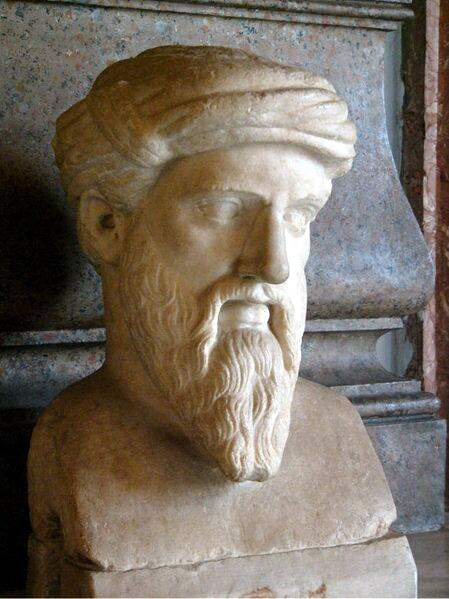
\includegraphics[width=0.4\textwidth]{photos/pythagoras.jpg}
    \end{center}
    \caption{\emph{Busto di Pitagora. Copia romana di originale greco. Musei Capitolini, Roma}.
    Original uploader was \emph{Galilea} at \url{http://de.wikipedia.org}.
    File used under the terms of the Creative Commons Attribution-Share Alike 3.0 Unported license.}
  \label{fig:bustofpythagoras}
\end{figure}
